\subsection{Оптоэлектронный классификатор изображений}
Идея создания гибридной оптоэлектронной сети для классификации основано на концепции, описанной в параграфе, посвящённом сжатия информации, в секции \ref{sec:OpticalCalcs}. Принципиальная схема представлена на рисунке \ref{ris:OEScheme}.
\begin{figure}[h]
	\centering{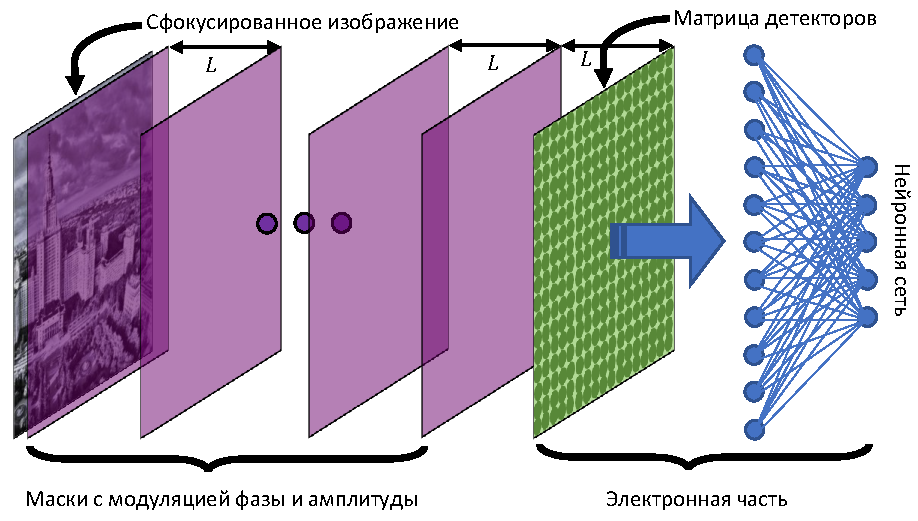
\includegraphics[width=1.0\linewidth]{figures/NetworkScheme.pdf}}
	\caption{Схема оптоэлектронной нейронной сети. $L$ - расстояние между слоями.}
	\label{ris:OEScheme}
\end{figure}
Излучение распространяется через модуляторы и попадает на матрицу детекторов. После регистрации интенсивностей детекторами, сигналы обрабатывается электронной нейронной сетью на компьютере. В качестве электронной модели была выбрана свёрточная архитектура ResNet18 \cite{he2016deep}, основанная на остаточных блоках. Слои свёртки  имеют маленькие ядра, что положительно сказывается на скорости работы. Эта модель может обрабатывать изображения любой размерности, поэтому будет удобно сравнивать нейронную сеть без оптической пред обработки и с ней.

\paragraph{Параметры модели}
Параметры модели были выбраны эмпирическим исходя из корректности численных расчётов распространения света и скорости обучения модели. Длинна волны -- $500$ нм, размер расчётной области -- $5$ мм, количество узлов вычислительной сетки по одной оси -- $300$ шт, размер неоднородности маски -- $50$ мкм, расстояние между масками -- $90.5$ мм, количество некогерентных реализаций для усреднения -- $7$ шт, количество модуляторов амплитуды и фазы -- $3$ шт. Детекторы моделировались функцией Гаусса с дисперсией -- $83$ мкм, а их количество равнялось -- $24 \times 24$. Пространственная когерентность принимала различные значения.

\paragraph{Подготовка данных}
В качестве набора размеченных изображений для классификации был выбран CIFAR10. Этот набор состоит из $10$-ти классов, по $6000$ изображений размером $32 \times 32$ пикселя в каждом классе. Примеры изображений представлены на рисунке \ref{ris:CIFAR10}.
\begin{figure}[h]
	\centering{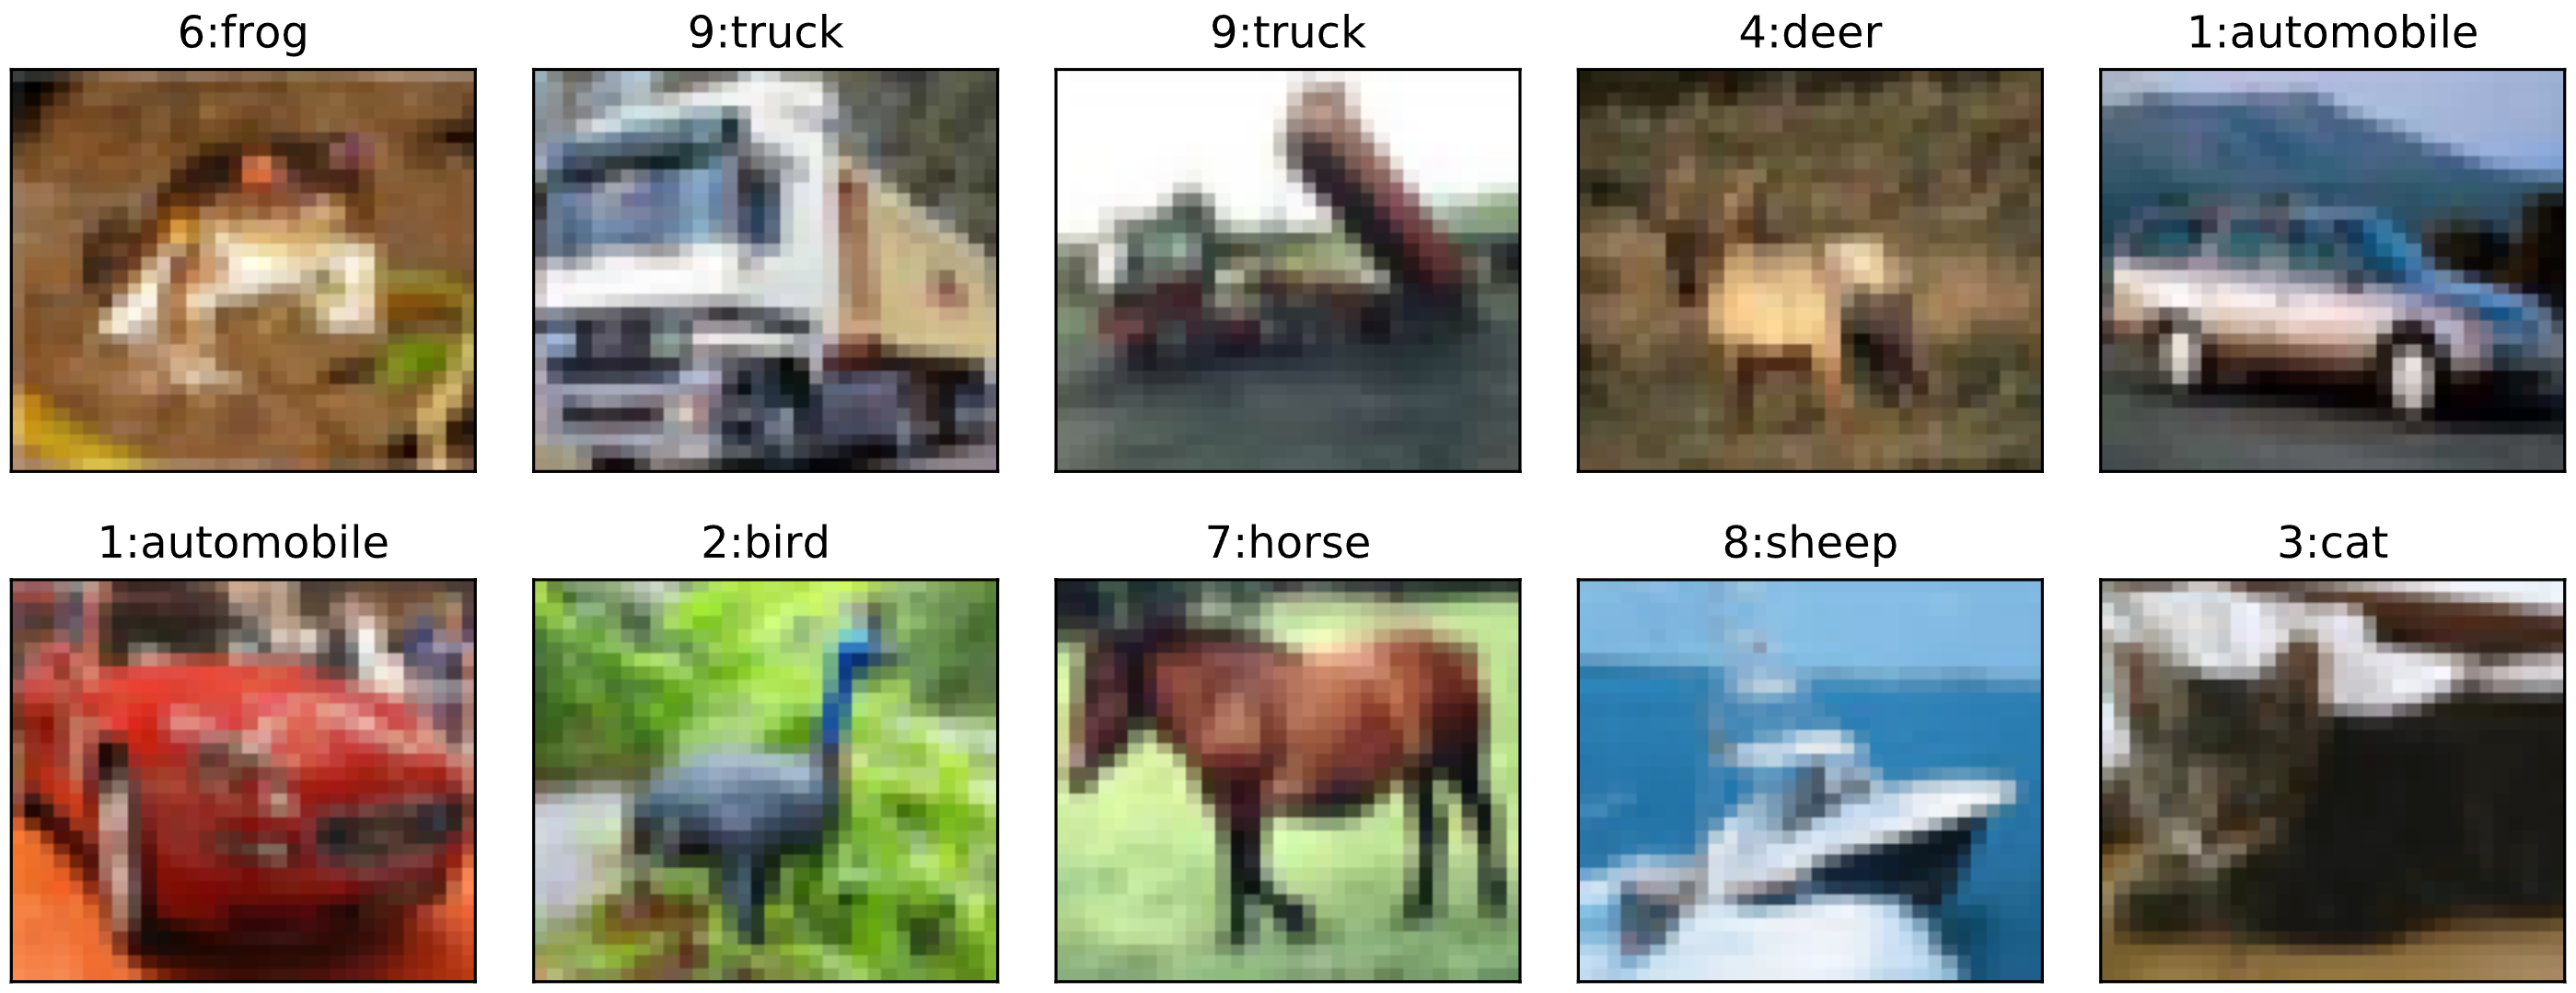
\includegraphics[width=1.0\linewidth]{figures/CIFAR10.png}}
	\caption{Примеры изображений набора CIFAR10.}
	\label{ris:CIFAR10}
\end{figure}
Изображения приводились к черно-белому формату и интерполировались до размера, соответствующего размеру вычислительной сетки, с помощью метода кубической интерполяции.

\paragraph{Обучение модели}
Модель обучалась с помощью алгоритма обновления весов RMSprop в два этапа. Данный алгоритм был выбран эмпирически. На первом этапе частота обучения (learning rate) была равна $0.01$, на втором - $0.0001$. Каждый этап состоял из $30$-ти эпох. Количество изображений в одном пакете данных (batch) тоже было выбрано эмпирически -- $22$. В качестве функции ошибки использовалась смесь средне квадратичной ошибки и кросс-энтропии в пропорции $0.39$ к $0.61$ соответственно.